\begin{frame}[fragile]{On-the-Fly Parameterization (OTFP) to Get $F$ from TAMD}
    \begin{tikzpicture}
        \pcuad{\textwidth}{\textheight}
        %\showcuad
        \path(se) 
            ++(0,1) node(text)[anchor=south east]{
                {\tiny \textcolor{blue!80!black}{CFA and E. Vanden-Eijnden {\em Chem Phys Lett} {\bf 547}:114 (2012)}}
            };
        \path(nw) 
            ++(0,-0.5) node(text)[anchor=west]{
                \textcolor{blue!80!black}{Basis-function expansion}
            }
            ++(0,-0.75) node(Fz)[anchor=west]{
                $\ds \tilde{F}(\zb) = \sum_k\lambda_k\phi_k(\zb)$
            }
            ++(0,-1) node(text2)[anchor=west]{
                \textcolor{red!80!black}{Error estimate}
            }
            ++(0,-0.8) node(Elambda)[anchor=west]{
                $\ds E(\lambdab) = \Big<\sum_j\left[\kappa[z_j-\theta_j(\xb)]-\frac{\partial \tilde{F}(\zb)}{\partial 
        z_j}\right]^2\Big>_{\rm TAMD}$
            }
            ++(3,1.25) node(min)[anchor=west]{
                \textcolor{green!80!black}{Minimize}
            }
            ++(1.5,1) node(dEdlambda)[anchor=west]{
                $\ds \frac{\partial E}{\partial \lambdab}=0$
            }
            ++(1.75,0) node(A)[anchor=west]{
                $\ds \uu{A}\lambdab = \uu{b}$
            }
            ++(1.75,0) node(lam)[anchor=west]{
                $\ds\lambdab = \uu{A}^{-1}\uu{b}$
            }
            ++(2.25,0) node(FF)[anchor=west]{
                $\ds \tilde{F}(\zb)$
            };
        \draw [->,thick,color=orange!80!black] (Elambda.north) -- (min.south);
        \draw [->,thick,color=orange!80!black] (min.north) -- (dEdlambda.south west);
        \draw [->,thick,color=orange!80!black] (dEdlambda.east) -- (A.west);
        \draw [->,thick,color=orange!80!black] (A.east) -- (lam.west);
        \draw [->,thick,color=orange!80!black] (lam.east) -- (FF.west);
        \path(wp) 
            ++(0,0) node(Anm)[anchor=west]
            {
                {\tiny $\ds A_{nm} = \frac{1}{2}\left<\sum_i\frac{\partial \phi_m(\zb)}{\partial z_i} 
        \frac{\partial \phi_n(\zb)}{\partial z_i}\right>_{\rm TAMD}$}
            }
            ++(0,-0.7) node(bm)[anchor=west]{
                {\tiny $\ds b_{m} = \left<\sum_i\frac{\partial \phi_m(\zb)}{\partial 
        z_i} \kappa[z_i-\theta_i(\xb)]\right>_{\rm TAMD}$}
            };
        
        \draw[<->,thick,color=green!80!black] (0.1\bbw,0.2\bbh) -- (0.5\bbw,0.2\bbh);
        \draw[->,thick,color=green!80!black] (0.3\bbw,0.2\bbh) -- (0.3\bbw,0.35\bbh);
        \draw[thick,color=orange!50!black] (0.4\bbw,0.2\bbh) -- (0.3\bbw,0.3\bbh);
        \draw[thick,color=orange!50!black] (0.3\bbw,0.3\bbh) -- (0.2\bbw,0.2\bbh);
        \draw[thick,color=green!80!black] (0.2\bbw,0.2\bbh) -- (0.2\bbw,0.18\bbh);
        \draw[thick,color=green!80!black] (0.4\bbw,0.2\bbh) -- (0.4\bbw,0.18\bbh);
        \draw[thick,color=green!80!black] (0.3\bbw,0.2\bbh) -- (0.3\bbw,0.18\bbh);
        \draw (0.3\bbw,0.15\bbh) node {$m$};
        \draw (0.2\bbw,0.15\bbh) node {$m-1$};
        \draw (0.4\bbw,0.15\bbh) node {$m+1$};
        \draw (0.32\bbw,0.32\bbh) node {1};
        \draw (0.35\bbw,0.29\bbh) node {$\phi_m$};
        
        \path(ep) 
            ++(0,0.5) node(plot)[graphics,anchor=north east]{
                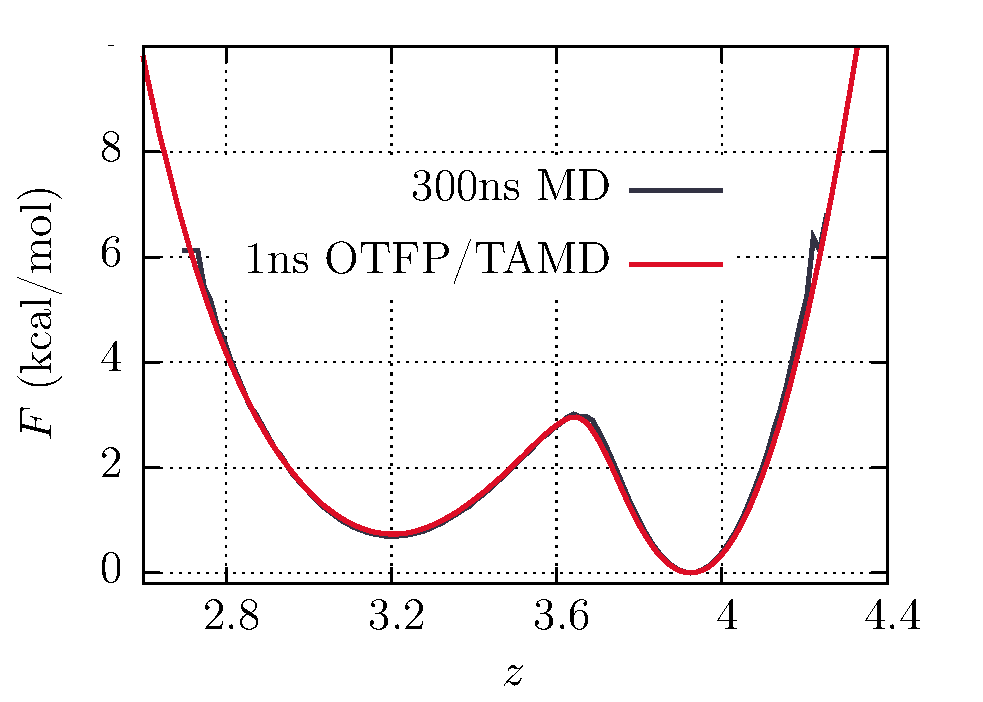
\includegraphics[width=0.45\textwidth]{otfpc4}
            }
            ++(0,0) node(config)[graphics,anchor=south east]{
                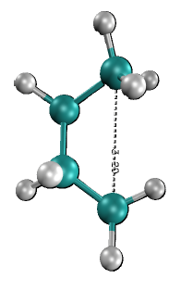
\includegraphics[width=0.16\textwidth]{butane}
            };
        \end{tikzpicture}
\end{frame}

